
\chapter{Orlin Algorithm} \label{chap:Orlin}

    Before delving into Orlin's algorithm, let's review the current state of the problem.  
    The Goldberg-Rao algorithm achieves what is called a \textit{weakly polynomial} time complexity, solving the problem in \(\log mU\) phases, each with a cost of \( O(\Lambda m \log(n^2/m)) \), where \( \Lambda = \min \{n^{2/3}, m^{1/2}\} \).  
    If we aim to solve the maximum flow problem with a \textit{strongly polynomial} time complexity, there is the King-Rao-Tarjan algorithm. However, this algorithm achieves a time cost of \( O(nm) \) only under the condition that \( m = \Omega (n^{1+\varepsilon}) \) for some \( \varepsilon > 0 \).  
    If the number of edges is insufficient, its cost is \( O(nm \log_{m / (n \log n)} n) \).  

    In the following algorithm, James B. Orlin proposes a solution that, by leveraging the Goldberg-Rao algorithm, manages to solve the maximum flow problem in \( O(nm) \) when \( m = O(n^{1+\varepsilon}) \). This makes it possible to solve the problem in strictly polynomial time for any values of \( n \) and \( m \), without being limited by edge capacities.


\section{Idea}

    The idea arises from several observations:\\
    The Goldberg-Rao algorithm operates through \textbf{increment phases} that take a \(\Delta\)-optimal flow and make it \(\Delta/2\)-optimal.  
    Furthermore, it is noted that \(\log_{8m} mU \leq 1 + \log U\); in fact, from now on, \(\log U\) increment phases will be considered.  
    If we set \(\Lambda = O(m^{1/2})\), we can observe that  
    \[
    \log U < m^{7/16} \implies \tilde{O}(m^{3/2} \cdot m^{7/16}) = \tilde{O}(m^{31/16})
    \]
    (the notation \(\tilde{O}\) ignores logarithmic factors).\\
    Delving deeper into the calculations, we observe  
    \[
    \tilde{O}(m^{31/16}) = O(m \cdot m^{15/16} \cdot \log(n^2/m)) = O(m \cdot n^{(16/15)^{15/16}} \cdot \log(n^2/m))
    \]
    since we are looking for an algorithm when \(m = O(n^{1+\varepsilon})\). If \(1+\varepsilon < 16/15\) and \(\log U < m^{7/16}\), we can achieve an optimal solution with a polynomial cost of \(O(nm)\) by using only the Goldberg-Rao algorithm.

    However, this is only true if the number of edges is sufficiently larger compared to the edge with the maximum capacity.  
    
    Hence, the idea of contracting and compacting the network arises to ensure the calculation of the maximum flow under optimal conditions.

    The algorithm presents two bottlenecks:
    \begin{enumerate}
        \item Creation of the compacted representation (more precisely, maintaining the transitive closure)
        \item Transitioning from the compacted flow to the extended flow.
    \end{enumerate}

\section{Fase di incremento}
If the Goldberg-Rao algorithm, in a sense, 'wraps' Dinic's Algorithm into a higher level of abstraction where the original graph is modified, Orlin does the same with Goldberg-Rao.

A higher level of increment phase is introduced, within which a slightly modified version of the Goldberg-Rao algorithm is executed.
So let's examine the input and output of each phase:

\begin{itemize}[itemsep=0.5ex]
    \item \textbf{Input}
    \begin{enumerate}
        \item a \textit{Flow} \(f\)
        \item a \textit{Residual Graph} \(G_f\), 
        \item an s-t cut \((S,T)\)
    \end{enumerate}
    Since with the flow and the residual graph, we can compose the residual function, when we consider the flow and the graph we can say to have also the residual function "r". \\
    We can represent the input as the tuple \((r, S, T)\).
    
    \item \textbf{Output}
    \begin{enumerate}
        \item a \textit{Flow} \(f'\)
        \item a \textit{Residual Graph} \(G_f'\)
        \item an s-t cut \((S', T')\) such that \(r'(S', T') \leq \frac{r(S, T)}{8m}\)
    \end{enumerate}
\end{itemize}

This phase is called the \(\Delta\text{-improvement phase}\), where \(\Delta = r(S, T)\). Alongside the parameter \(\Delta\), a parameter \(\Gamma\) is introduced, where \(\Gamma \leq \Delta\), which will be used to create the \(\Gamma\)-compact network.

Depending on the conditions, the \(\Delta\)-improvement will be executed either on the original network \(G\) or on the \(\Gamma\)-compact network \(G^c\), which we will introduce later.
\newpage

\section{$\Delta$-abundant e grafo di abbondanza}
In questa sezione viene presentato il concetto di \textbf{Abbondanza}.

\begin{definition}[$\Delta$-abundant arc]
    Let $\Delta = r(S,T)$ then any edge $(i,j)$ is said $\Delta$-abundant if $r_{ij} \ge 2\Delta$ 
     
\end{definition}
\begin{lemma}
    \label{ab4ever}
    Let $(r,S,T)$ be the input for a $\Delta\text{-}improvement\ phase$. If the edge  $(i,j)$ is abundant before the phase then it will be abundant for for all subsequent phases.
\end{lemma}
\begin{proof}
    Since
    $\Delta' \le \frac{\Delta}{8m} $ and recalling that $r_{ij} \ge 2\Delta $ it follows that 
    allora \[r'_{ij} \ge r_{ij}-\Delta \ge\Delta\ge  2\Delta'\]
\end{proof}

\begin{definition}[Abundance Graph]
    Given a network $G$, its \textbf{Abundance Graph} $G^{ab}$ is defined as: 
    \[G^{ab} := (N(G), \{(i,j)| (i,j)\in E(G)\land r_{ij}\ge 2\Delta\})\]
\end{definition}

\begin{obs}
    By lemma \ref{ab4ever}, as iterations proceed, the abundant graph can only acquire new edges, never lose them.
\end{obs}

The abundant graph has two purposes: 
\begin{enumerate}
    \item All cycles formed by abundant edges are \textit{contracted} into a single node.
    \item All nodes adjacent only to abundant edges (or edges with capacity that is too small) are \textit{compacted}.
\end{enumerate}

    Additionally, the algorithm maintains the transitive closure of all nodes connected by an \textbf{abundant path}, meaning a path composed only of abundant edges.\\
    If there exists an abundant path between nodes \( i \) and \( j \), this is indicated as \( i \implies j \), and the information is stored in an \textbf{M}$_{n \times n}$ matrix, where at position \textbf{M}$_{i,j}$ is the node that precedes \( j \) in the path starting from \( i \). If multiple paths are created during the iterations, the first one found is kept.

    The transitive closure can be maintained in time \( O(nm) \) using Italiano's algorithm. 
    In this way, it is always possible to reconstruct an abundant path \( P \) in \( O(|P|) \) (we will see later that contracting the graph does not prevent this nor does it alter its cost).

\newpage
\section{Contractions of abundant graph}
Let's now see how to exploit the abundant graph to contract the graph on which we calculate the max-flow and make the algorithm more efficient.

We analyze three different examples of contractions:

Suppose there are two nodes \(i\) and \(j\) such that \(r_{ij} \geq 2\Delta\) and \(r_{ji} \geq 2\Delta\).
We can contract the two nodes into a single one, preserving the edges of both.

\[\begin{tabular}{ccc}
    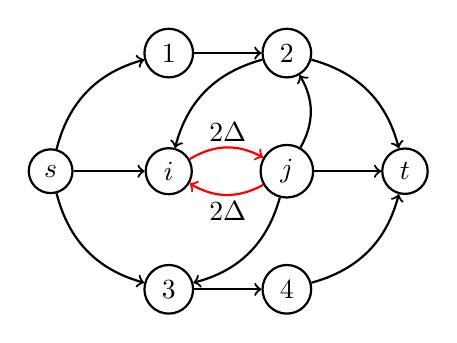
\begin{tikzpicture}[node distance={15mm}, thick , main/.style = {draw, circle}] 
    % Disegna i nodi del grafo
    

    \node[main] (0) {$s$};
    \node[main] (3) [right of= 0 ] {$i$};
    \node[main] (4) [right of=3] {$j$};
    \node[main] (1) [below of = 3 ] {3};
    \node[main] (2) [above of = 3] {$1$};
    
    \node[main] (6) [above of=4] {$2$};
    \node[main] (5) [below of=4] {$4$};
    \node[main] (7) [right of=4] {$t$};
    % Disegna gli archi orientati
    \draw[->] (0) [bend right] to (1);
    \draw[->] (0) [bend left] to (2);
    \draw[->] (0) to (3);
    \draw[->] (3) [red, bend left] to (4);
    \node at (2.25,0.5) {$2\Delta$};
    \node at (2.25,-0.5) {$2\Delta$};
    \draw[->] (4) [red, bend left] to (3);
    
    \draw[->] (2) to (6);
    \draw[->] (4)[bend left] to (1);
    \draw[->] (4)[bend right] to (6);
    \draw[->] (6)[bend right] to (3);
    \draw[->] (4) to (7);
    \draw[->] (1) to (5);
    \draw[->] (6)[bend left] to (7);
    \draw[->] (5)[bend right] to (7);


\end{tikzpicture}&\begin{tikzpicture}
    \node {$\implies$};% Freccia verso destra
    \node at (0,1.4) {};
    \node at (0,-1.6) {};
\end{tikzpicture}  &
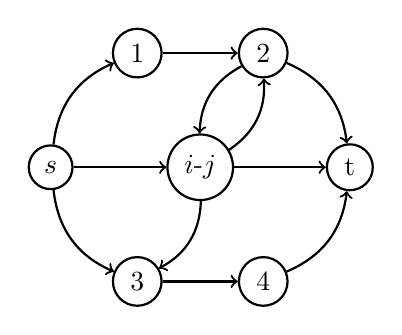
\begin{tikzpicture}[node distance={19mm}, thick , main/.style = {draw, circle}] 
    % Disegna i nodi del grafo
    
    
    \node[main] (m)  {$i$-$j$};
    \node[main] (0) [left of = m ]{$s$};
    \node[main] (1) at (-0.8,1.45) {1};
    
    \node[main] (2) at (0.8,1.45) {$2$};

    \node[main] (3) at (-0.8,-1.45) {$3$};
    \node[main] (4) at (0.8,-1.45) {$4$};

    \node[main] (5) [right of = m] {t};
    % Disegna gli archi orientati

    
    \draw[->] (0) to (m);
    \draw[->] (0)[bend left] to (1);
    \draw[->] (0)[bend right] to (3);

    \draw[->] (1) to (2);

    \draw[->] (2)[bend right] to (m);
    \draw[->] (m)[bend right] to (2);
    \draw[->] (m)[bend left] to (3);
    \draw[->] (2)[bend left] to (5);
    \draw[->] (m) to (5);
    \draw[->] (3) to (4);  
    \draw[->] (4)[bend right] to (5);

\end{tikzpicture}
\end{tabular}\]

Since there are no reverse edges for the external edges, it is possible to contract external edges under the sole condition that they are abundant.

\[\begin{tabular}{ccc}
    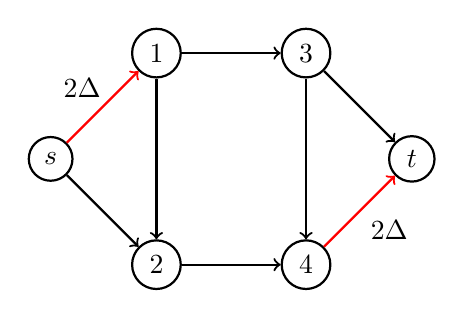
\begin{tikzpicture}[node distance={19mm}, thick , main/.style = {draw, circle}] 
    % Disegna i nodi del grafo
    
    \node[main] (0) {$s$};
    \node[main] (1) [above right of = 0] {1};
    \node[main] (2) [below right of = 0] {2};
    \node[main] (3) [right of = 1] {3};
    \node[main] (4) [right of = 2] {4};
    \node[main] (5) [below right of = 3] {$t$};
    
    \draw[->] (0) [red] to (1);
    \draw[->] (1) to (3);
    \draw[->] (0) to (2);
    \draw[->] (2) to (4);
    \draw[->] (3) to (5);
    \draw[->] (4) [red] to (5);
    \draw[->] (1) to (2);
    \draw[->] (3) to (4);

    \node at (0.4,0.9) {$2\Delta$};
    \node at (4.3,-0.9) {$2\Delta$};

\end{tikzpicture}&\begin{tikzpicture}
    \node {$\implies$};% Freccia verso destra
    \node at (0,1.4) {};
    \node at (0,-1.6) {};
\end{tikzpicture}  &
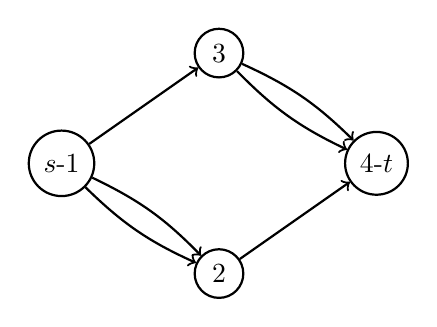
\begin{tikzpicture}[node distance={19mm}, thick , main/.style = {draw, circle}] 
    % Disegna i nodi del grafo
    \node[main] (0) {$s$-$1$};
    \node[main] (3) at (2,1.4) {$3$};
    \node[main] (2) at (2,-1.4) {$2$};
    \node[main] (4) at (4,0) {4-$t$};

    \draw[->] (0) to (3);
    \draw[->] (0) [bend left = 10] to (2);
    \draw[->] (0) [bend right = 10] to (2);
    
    
    \draw[->] (2) to (4);
    \draw[->] (3) [bend left = 10] to (4);
    \draw[->] (3) [bend right = 10] to (4);
    

\end{tikzpicture}
\end{tabular}\]

And so all the abundant cycles

\[\begin{tabular}{ccc}
    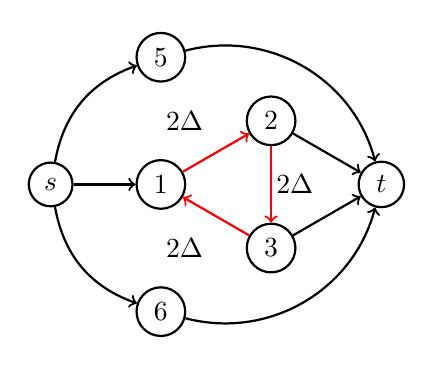
\begin{tikzpicture}[node distance={18mm}, thick , main/.style = {draw, circle}] 
    % Disegna i nodi del grafo
    
    \node[main] (0) {$s$};
    \node[main] (1) at (1*1.4,0) {1};
    \node[main] (2) at (2*1.4,0.577*1.4) {2};
    \node[main] (3) at (2*1.4,-0.577*1.4) {3};
    \node[main] (4) at (3*1.4,0) {$t$};
    \node[main] (5) at (1*1.4,1.154*1.4) {$5$};
    \node[main] (6) at (1*1.4,-1.154*1.4) {$6$};

    \draw[->] (0) [bend left] to (5);
    \draw[->] (0) [bend right] to (6);
    \draw[->] (0)  to (1);
    \draw[->] (1)[red]  to (2);
    \draw[->] (2)[red]  to (3);
    \draw[->] (3)[red]  to (1);
    \draw[->] (2)  to (4);
    \draw[->] (3)  to (4);
    \draw[->] (5) [bend left = 45] to (4);
    \draw[->] (6) [bend right = 45] to (4);

    \node at (3.1,0) {$2\Delta$};
    \node at (1.7,0.577*1.4) {$2\Delta$};
    \node at (1.7,-0.577*1.4) {$2\Delta$};
    

\end{tikzpicture}&\begin{tikzpicture}
    \node {$\implies$};% Freccia verso destra
    \node at (0,1.4) {};
    \node at (0,-1.6) {};
\end{tikzpicture}  &
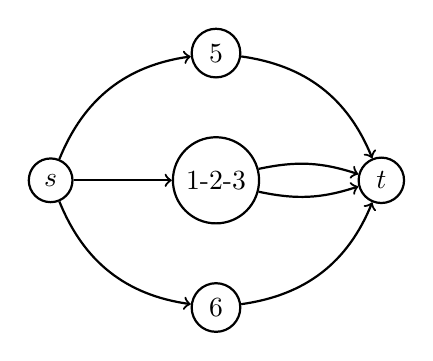
\begin{tikzpicture}[node distance={19mm}, thick , main/.style = {draw, circle}] 
    % Disegna i nodi del grafo
    \node[main] (0) {$s$};
    \node[main] (1) at (1.5*1.4,0) {1-2-3};
    \node[main] (5) at (1.5*1.4,1.154*1.4) {$5$};
    \node[main] (6) at (1.5*1.4,-1.154*1.4) {$6$};
    \node[main] (4) at (3*1.4,0) {$t$};

    \draw[->] (0) [bend left] to (5);
    \draw[->] (5) [bend left] to (4);
    \draw[->] (0) [bend right] to (6);
    \draw[->] (6) [bend right] to (4);

    \draw[->] (0) to (1);
    \draw[->] (1) [bend left= 15] to (4);
    \draw[->] (1) [bend right = 15] to (4);

\end{tikzpicture}
\end{tabular}\]

\begin{obs}
    It is possible that when the contracted graph is expanded again, the flow conservation law may be violated.
\end{obs}
    However, this violation is minor, at most \(2\Delta\) units; thus, as shown by Goldberg and Rao, the contraction, expansion, and adjustment for flow conservation can be performed in \(O(m)\) time.

\section{How to compact network}

In addition to the contraction of the graph, another transformation is necessary: the \textit{compaction}. To obtain a compact graph, we first demonstrate how to achieve an intermediate version, namely the \textbf{strongly compact network}.

It is important to understand the difference between contracting and compacting:

In contraction, a single node is created that represents the abundant cycle, and the original edges not belonging to the cycle are preserved. However, when compacting a graph, a node that has all adjacent edges abundant is \underline{eliminated}, and the outgoing edges are consequently replaced by pseudo-edges.
\[\begin{tabular}{ccc}
    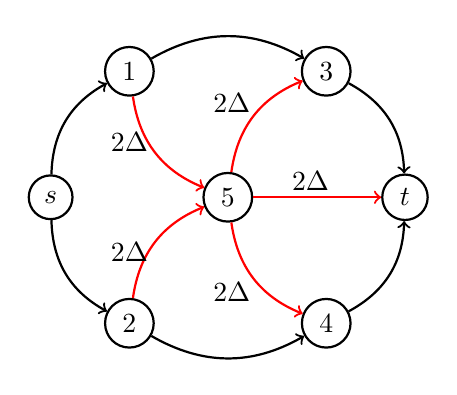
\begin{tikzpicture}[node distance={18mm}, thick , main/.style = {draw, circle}] 
    % Disegna i nodi del grafo
    
    \node[main] (0) {$s$};
    \node[main] (1) at (1, 1.6) {1};
    \node[main] (2) at (1, -1.6) {2};
    \node[main] (3) at (3.5, 1.6) {3};
    \node[main] (4) at (3.5, -1.6) {4};
    \node[main] (6) at (2.25,0) {5};
    \node[main] (5) at (4.5, 0) {$t$};

    \draw[->] (0)[bend left] to (1);
    \draw[->] (0)[bend right] to (2);
    \draw[->] (1)[bend left] to (3);
    \draw[->] (2)[bend right] to (4);
    \draw[->] (4)[bend right] to (5);
    \draw[->] (3)[bend left] to (5);

    \draw[->] (1)[red, bend right] to (6);
    \draw[->] (6)[red, bend right] to (4);
    \draw[->] (6)[red, bend left] to (3);
    \draw[->] (2)[red, bend left] to (6);
    \draw[->] (6) [red] to (5);

    \node at (3.3,0.2) {$2\Delta$};
    \node at (2.3,1.2) {$2\Delta$};
    \node at (2.3,-1.2) {$2\Delta$};

    \node at (1,.7) {$2\Delta$};
    \node at (1,-.7) {$2\Delta$};
    

\end{tikzpicture}&\begin{tikzpicture}
    \node {$\implies$};% Freccia verso destra
    \node at (0,1.4) {};
    \node at (0,-1.95) {};
\end{tikzpicture}  &
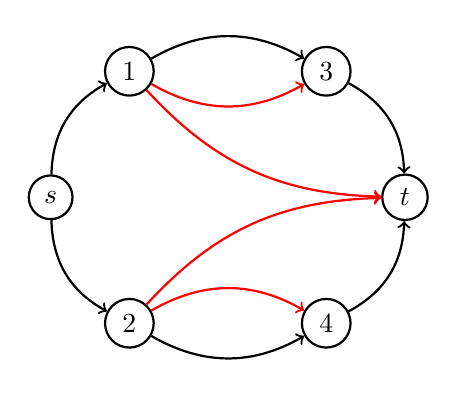
\begin{tikzpicture}[node distance={19mm}, thick , main/.style = {draw, circle}] 
    % Disegna i nodi del grafo
    \node[main] (0) {$s$};
    \node[main] (1) at (1, 1.6) {1};
    \node[main] (2) at (1, -1.6) {2};
    \node[main] (3) at (3.5, 1.6) {3};
    \node[main] (4) at (3.5, -1.6) {4};
    \node[main] (5) at (4.5, 0) {$t$};

    \draw[->] (0)[bend left] to (1);
    \draw[->] (0)[bend right] to (2);
    \draw[->] (1)[bend left] to (3);
    \draw[->] (2)[bend right] to (4);
    \draw[->] (4)[bend right] to (5);
    \draw[->] (3)[bend left] to (5);

    \draw[->] (1)[red, bend right] to (3);
    \draw[->] (2)[red, bend left] to (4);
    \draw[->] (2)[red, bend left = 23] to (5);
    \draw[->] (1)[red, bend right = 23] to (5);


\end{tikzpicture}
\end{tabular}\]

The following algorithm has a time complexity of \(O(m + |E^{sc}|)\) since pseudo-edges can be constructed in \(O(1)\) time, given that the transitive closure is dynamically preserved.

\begin{definition}[Strongly compact network]

    We define the \textbf{Strongly compact} as \(G^{sc} =(N^{sc}, E^{sc})\) originated from the network \(G\):
    \begin{enumerate}
        \item Contract the graph of all abundant cycles and the external abundant edges.\\
        Let \((r,S,T)\) be the input after contraction.
        \item Let \(N^{sc}\subseteq N(G)\) be the set of nodes that are adjacent to at least one non-abundant edge.\\
        We will refer to \(N(G)\setminus N^{sc}\) as the set of \textit{strongly compactible} nodes.
        \item We define the edges as \(E^{sc} = E^1 \cup E^2\) where:\\
        \(E^1 = \{(i,j): i\in N^{sc}\land j\in N^{sc}\land (i,j)\in E(G)\}\)\\
        \(E^2 = \{(i,j): i\in N^{sc}\land j\in N^{sc}\land i\implies j\}\)\\
        Thus, we have original edges in \(E^1\) and pseudo-edges that derive from the abundant paths.
    \end{enumerate}
\end{definition}

When we contract the graph, we are sure that if the flow routed in the contracted graph is less than a certain parameter \(\Delta\) with which we contracted the graph, then that flow is also adaptable on the original one. The following theorem shows us that the same is true for strongly compact graphs.
\newpage

\begin{theorem}[$f_{max} = f_{max}^{sc}$]

    \label{fmaxfsc}
    Let \(f_{max}\) be the maximum flow in the network \(G\) and let \(f_{max}^{sc}\) be the maximum flow in \(G^{sc}\). Then 
    \[f_{max} = f_{max}^{sc}\]
\end{theorem}

\begin{proof}
    We have already shown that any flow in \(G^{sc}\) can be rerouted in \(G\).
    If we take a flow in \(G\), it can be routed in \(G^{sc}\) using the \textbf{flow decomposition} to obtain from \(f\) a set of paths that differ by at least one edge,
    \[f := \{P^0, P^1, ..., P^k\}\]
    We can further subdivide each \(P^a\in f\) into subpaths \[P^{a}_{i\rightarrow j}| i\in N^{sc}\land j\in N^{sc}\land \forall q \in P^a_{i\rightarrow j}, q\not = i \land q\not = j \implies q\in N\setminus N^{sc}\] 
    At this point, we replace each \(P^{a}_{i\rightarrow j}\) in \(G\) that is not entirely contained in \(G^{sc}\) with the corresponding pseudo-edge \((i,j)\).

\end{proof}



\section{From sc-compact to $\Gamma$-compact}
Il grafo sc-compact non è abbastanza compattato per raggiungere il costo desiderato. Per compattarlo ulteriormente dovremmo utilizzare un parametro \gmm per scegliere quali nodi compattare e da quali archi trasferire capacità residua.
La scelta del parametro \gmm\ verrà mostrata in seguito.
Prima di proseguire è importante distinguere diversi tipi di archi.
\begin{definition}[Classificazioni di capacità]
    Un arco $(i,j)$ rispetto a $\Gamma$ ha:
    \begin{enumerate}
        \item \textbf{small capacity} se $u_{ij}+u_{ji} < \Gamma/(64m^3)$
        \item \label{media}\textbf{medium capacity} se $\Gamma/(64m^3) \le u_{ij}+u_{ji}\ \land$\\ $r_{ij} < 2\Delta \land r_{ji} < 2\Delta $
        \item \textbf{abundant capacity} se $r_{ij} \ge 2\Delta$ 
        \item \textbf{antiabundant capacity} se $(j,i) \in E^{ab} \lor\ (i,j)$ è un arco esterno non abbondante.
    \end{enumerate}
    Dove $E^{ab}$ e $E^{-ab}$ rappresentano rispettivamente l'insieme degli archi abbondanti e anti abbondanti all'inizio dell'improvement phase.

   
    
\end{definition}
\begin{obs}
    Dato che abbiamo contratto i cicli abbondanti se $(i,j)\in E^{ab}\implies (j,i)\not \in E^{ab}$
\end{obs}


Un altro strumento necessario per decidere quali nodi compattare è la funzione \textit{potenziale}
\begin{definition}[Potential function]

    Dato un nodo $j\in N$ una funzione di capacità residua $r$ e un sottoinsieme di archi adiacenti a $j$ $\tilde{E}$  possiamo definire la funzione potenziale come: 
    \[\Phi (j, r, \tilde{E}) = \sum_{(i,j)\in \tilde{E}} r_{ij}-\sum_{(j,i)\in \tilde{E}} r_{ji}\] 
\end{definition}

    È secondo questi parametri che in ogni improvement phase vengono distinti i nodi che si possono compattare da quelli che non possono essere compattati. Queste due distinzioni prendono il nome rispettivamente di nodi \gmm-compactible e nodi \gmm-critical. 
    \begin{definition}[$\Gamma$-critical e $\Gamma$-compactible]
        
        Un nodo j si dice \textbf{$\Gamma$-critical} se è adiacente almeno ad un arco \gmm-medio oppure se $|\Phi (j, r, E^{-ab})| > \Gamma/(16m^2)$.

        Se un nodo non è $\Gamma$-critical allora si dice \textbf{$\Gamma$-compactible}.

        \vspace*{7pt}
        Dato un network $G$ definiamo il \gmm\-compact network di $G$ come \[G^c := (N^c, E^c)\]
        Dove $N^c$ sono tutti e soli i nodi \gmm-critical mentre $E^c$ l'insieme di archi che definiremo in seguito.
    \end{definition}
    Per costruire il $\Delta$-compact network vengono iterativamente trasferite unità di capacità residue di vari path a pseudo archi. 
    l'idea è quella di sottrarre capacità a dei percorsi che collegano due nodi $i,j\in N$ per passarla all'arco (o pseudo arco) $(i,j)$ e poter ulteriormente compattare il grafo.
    Ovviamente però questi pseudo archi sono solo parte di quelli che compongono $E^c$ che potremmo definire come 
    \[E^c = E^1\cup E^2 \cup E^3\]
    $E^1 = \{(i,j) | i,j\in N^c \land (i,j) \in E(G)\}$ dunque gli archi originali che collegano due nodi \gmm-critici\\
    $E^2 = \{(i,j) | i,j\in N^c \land i\implies j\}$ ovvero gli archi abbondanti 

    Il seguente lemma mostra come se scelti secondo un appropriato criterio, il trasferimento di flusso non riduce la capacità di nessun (S,T) cut e dunque preserva il max flow calcolabile.
    \begin{lemma}[label = {ftsafe}]{Flow transfer safety}{}
        Sia $(S,T)$ un s-t cut in $G$ con $r(S,T)\le \Delta$, e sia $A' = E^{-ab}.$\\
        Supponiamo che esista $P\subseteq A'$ un path da $i\rightarrow j$ e che $(i,j)\in A'$. \\
        Se $r'$ è la nuova funzione di capacità residua ottenuta spostando $\delta$ unità di capacità residua da $P$ a $(i,j)$, allora possiamo affermare che:
        \begin{enumerate}
            \item $\forall k\in N(G),\ \Phi(k,r',A') = \Phi(k,r,A') $
            \item $r'(S,T) = r(S,T)$
        \end{enumerate}
        
    \end{lemma}
        \begin{proof} \begin{enumerate}
                \item Il primo punto è intuitivo in quanto per ogni nodo in $P$ diverso da $i$ e $j$ sto sottraendo la stessa capacità residua sia in entrata che in uscita, mentre nei nodi $i$ e $j$ le sommatorie di $\Phi$ rimangono identiche.
                \item Il secondo punto è banale se $|P|= 1$ dunque consideriamo $|P|\ge 2$. Definiamo $P = p_1, ..., p_k$, $p_1 \in S$ e almeno un $p_q\in T$.\\
                    Dato che abbiamo stabilito che $r(S,T) \le \Delta$ e che $P\subseteq A'$ ci troviamo sicuramente in una situazione di questo tipo:
                    \[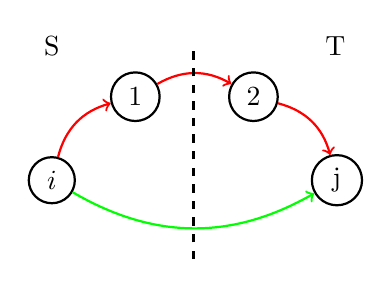
\begin{tikzpicture}[node distance={15mm}, thick , main/.style = {draw, circle}] 
                        % Disegna i nodi del grafo
                        \node[main] (0) {$i$};
                        \node[main] (1) [above right of = 0] {1};
                        \node[main] (2) [right of = 1] {2};
                        \node[main] (3) [below right of = 2] {j};
                        \node at (0,1.7) {S};
                        \node at (3.6,1.7) {T};
    
                        \draw[->] (0) [red, bend left] to (1);
                        \draw[->] (1) [red, bend left] to (2);
                        \draw[->] (2) [red, bend left] to (3);
                        \draw[->] (0) [green, bend right] to (3);
    
                        \draw[dashed] (1.8,-1) -- (1.8,1.7);
                    \end{tikzpicture}\]
                    In quanto se un arco di $P$ passasse da T a S violerebbe $r(S,T)\le \Delta$ dato che $\forall (a,b)\in A'(\Delta),\ r_{ab} > 2\Delta \land r_{ba}\ge 2\Delta$, avremmo che
                    \[\begin{tikzpicture}[node distance={15mm}, thick , main/.style = {draw, circle}] 
                        % Disegna i nodi del grafo
                        \node[main] (0) {$i$};
                        \node[main] (1) [above right of = 0] {1};
                        \node[main] (2) at (3.8,0) {2};
                        \node[main] (3) [below right of = 0] {j};
                        \node at (0,1.7) {S};
                        \node at (3.6,1.7) {T};
    
                        \draw[->] (0) [red,bend left] to (1);
                        \draw[->] (1) [red,bend left] to (2);
                        \draw[->] (2) [red,bend left] to (3);
                        \draw[->] (3) [thick = 1.5, darktangerine, bend left] to (2);
                        \draw[->] (0) [green, bend right] to (3);
    
                        \draw[dashed] (1.8,-1.7) -- (1.8,1.7);
                        \node at (2.4, -.4) {\text{\color{darktangerine}{$2\Delta$}}};
                    \end{tikzpicture}\]
                Una volta appurato ciò risulta evidente che il trasferimento di capacità residua non influenza la capacità residua del taglio. \QED
            \end{enumerate}
        \end{proof}
    Notiamo dunque che:
    \begin{definition}
        {Transferrable residual capacity}{}
        Per poter trasferire $\delta$ capacità da un path $P$ da $i\rightarrow j$ all'arco $(i,j)$ è necessario che:
        \begin{enumerate}
            \item $|P|\ge 2$
            \item $r(P) > 0$
            \item $P\subseteq A'$
       
        In oltre quando creeremo il \gmm\ compact network saranno essenziali anche i seguenti requisiti
        \item $i,j \in N^c$
        \item $P\setminus \{i,j\} \subseteq N(G) \setminus N^c$
    \end{enumerate}
    \end{definition} 
    La capacità che viene trasferita da è $\delta = r(P) = \min_{(a,b)\in P} r(a,b)$, dunque ogni volta almeno un arco anti-abbondante viene saturato. 
    Se esiste un path $P\subseteq A'\ da\ i\rightarrow j $ ma $(i,j)\not \in E(G)$ allora viene creato come pseudo arco. 
    Sono proprio questi Pseudo archi antiabbondanti che formeranno $E^3$. 
    Analizziamo ora la procedura per trasferire tutte le capacità residue necessarie a formare $E^3$ e restituirne l'insieme di archi
    con le relative capacità residue $r^c_{ij} \forall (i,j)\in E^3$

\begin{algorithm}
    \caption{\textit{Improve-approx-2(r,S,T)}}
    \label{imrAprx}
    \begin{algorithmic}[1]
        \State sia $G^c := \{n | n\in N(G)\land \Gamma\text{-critical}(n)\}$
        \State sia $H := \{(i,j)| (i,j)\in E^{-ab}\land i \not \in G^c \lor j \not \in G^c\}$
        \State $\forall (i,j)\in H,\ q_{ij} = r_{ij}$
        \While{H $\not = \varnothing$}
            \State seleziona $i \in H | \nexists (j,i) \in H$:
            \State P = $DFS(i, l)$ s.t $l\in N^c \lor \nexists (l,k)\in H$ \Comment{usa la DFS per un path da $i$ a $l$}
            \State sia $\delta = \min_{(a,b)\in P}q_{ab}$
            \If{$i,l \in N^c$} 
                \State $A^3 = A^3 \cup {(i,l)}; r^c_{il} += \delta$
            \EndIf
            \State $\forall (a,b) \in P,\ q_{ab} -= \delta$
            \State $H = H- \{(a,b) | q_{ab} = 0\}$ 
        \EndWhile 
    \end{algorithmic}
\end{algorithm}

Nel passaggio 6 viene creato, utilizzando una \textit{deep first search} un percorso dal nodo scelto $i$ fino ad uno $l$ che soddisfi certi requisiti.
Da notare con attenzione che \textbf{non è garantito} che $i$ e $l$ siano \gmm-critical e dunque è possibile che tale percorso (che esiste sempre) venga scartato.

Quando un percorso viene scartato si dice che $\delta$ capacità è stata \textbf{persa}. 
Dunque il max flow nel grafo \gmm-compact è inferiore a quello ottimale, tuttavia il seguente lemma mostra che esiste un bound a questa capacità residua \textit{persa}.
\begin{lemma}[Bound to \gmm-compact lose capacity] \label{boundlose}
    Sia $f_{max}$ il max-flow calcolato in $G$, il network originale, e $f^*$ quello calcolato in $G^c$, il network compattato creato dalla \nameref{algotrans}.
    Allora si ha che:
    \[f^*\le f_{max} \le f^* + \Gamma/16m\]
    ovvero il flusso massimo calcolato in $G^c$ è sottostimato di al più $\Gamma/16m$.
\end{lemma}
\begin{proof}
    Per essere scartato, un percorso deve iniziare o terminare in un nodo \gmm-compactible ovvero un nodo $j$ non adiacente ad un arco medio tale che:
    \[|\Phi (j, r, E^{-ab})| =\left | \sum_{(i,j)\in E^{-ab}} r_{ij}-\sum_{(j,i)\in E^{-ab}} r_{ji}\right |\le \Gamma/16m^2\]
    Tuttavia un nodo non critical per essere scelto deve avere solo archi entranti o solo archi uscenti a seconda di quale estremo del path stiamo parlando.
    Possiamo quindi stimare che la capacità massima di un certo path $P_s$ scartato sia $r(P_s) \le  \Gamma/16m^2$ ovvero il valore residuo massimo raggiungibile da un arco estremo a $P_s$.
    Dato quindi che possono esistere al massimo $n$ di questi percorsi allora abbiamo che: 
    \[n\cdot \Gamma/16m^2 \le m \cdot \Gamma/16m^2 = \Gamma/16m\]
    Dunque la massima capacità che viene persa nella creazione di $G^c$ è proprio $\Gamma/16m$.
\end{proof}

Dobbiamo ora assicurarci che un flow calcolato in $G^c$ che chiameremo $\alpha$-ottimale, sia trasferibile nel Network originale $G$.

Sia $f'$ il flow calcolato in $G^c$ e rappresentiamo con $f$ la trasposizione di $f'$ in $G$:\\
Se $f'_{i,j}> 0\land (i,j) \in E(G)\implies f_{i,j} = f'_{i,j}$ basta riportarlo così com'è.
se $f'_{i,j}> 0\land i \Rightarrow j \implies$ si tratta del compattamento di un path abbondante e per ripristinare il flusso basta usare la matrice di transitività.
Il caso più interessante rimane quello che si verifica quando dobbiamo trasporre il flusso da uno pseudo-arco di archi abbondanti ai path che lo hanno generato.
Infatti è importante ricordare che lo la capacità dello pseudo-arco è la somma delle capacità residue dei path che sono strati trasferiti in precedenza.
Tenere traccia di tutti i path trasferiti risulterebbe troppo inefficiente, tuttavia utilizzando gli alberi dinamici possiamo potenziare l'algoritmo precedentemente utilizzato per fare in modo di mantenere un record con tutte le operazioni effettuate sull'albero.
In questo modo è possibile, consultando il record a ritroso, ricostruire in tempo $k\log n$ (dove $k$ è  il numero di operazioni sul link-cut tree) le capacità trasferite dalla procedura in maniera sequenziale, potendo così adattare la giusta porzione di flusso in ogni arco.

Studiamo ora l'adattamento dal punto di vista dell'$(S,T)$-$cut$:\\
Sia $(S',T')$ un cut in $G[r]$ e supponiamo che non esistano archi abbondanti da $S$ a $T$,
un taglio $(S^c,T^c)$ in $G^c$ di dice \textbf{indotto da}  $(S',T')$ se: \[(S^c, T^c) := (S'\cap N(G^c), T'\cap N(G^c))\]
Viceversa un taglio in $G^c$ si dice indotto da uno in $G[r]$ se composto come segue:
\[\begin{array}{l}
    S':=\{n | n\in S^c\lor \exists m \in S^c,\ m \implies n\}\\
    T' = N(G)\setminus S'
\end{array}\]

\begin{obs}{}{}
    Osserviamo che se un $(S',T')$ è indotto da  $(S^c,T^c)$ allora  $(S^c,T^c)$ è indotto da $(S',T')$.
        \[(S',T')\leftarrow(S^c,T^c)\implies (S^c,T^c)\leftarrow(S',T')\]

    Non è vero il contrario in quanto diversi cut su $G[r]$ possono indurre lo stesso $(S^c,T^c)$.
\end{obs}

\begin{lemma}{}{}
    Supponiamo che $(S',T')$ sia un cut in $G[r]$ e che non esistano archi abbondanti da $S$ a $T$.
    Se $(S^c,T^c)$ è indotto da $(S',T')$ allora \[ r(S^c,T^c) \le r(S',T')\le r(S^c,T^c)+\Gamma/16m\]
\end{lemma}
\begin{proof}
    Sappiamo che gli archi originali in $E^1$ contribuiscono in egual misura sia in $(S^c,T^c)$ che in $(S',T')$, quelli abbondanti non sono presenti per ipotesi e dunque rimangono solo quelli in $E^3$.
    dividiamo path calcolati dalla \nameref{algotrans} come $P\cup Q$ dove $Q$ sono quelli che alla fine vengono scartati.
    Dal lemma \ref{ftsafe} sappiamo che trasferire la capacità non influenza la capacità del taglio. Quindi gli unici archi che possono influenzare la capacità residua restano quelli in $Q$.
    Ma sappiamo dal \cref{boundlose} che:
    \[\sum_{p\in Q}r(p)\le \Gamma/16m\]\QED
\end{proof}


Dai precedenti lemmi possiamo quindi giungere all'asserzione del seguente teorema
\begin{theorem}{}{}
    Sia $y$ un $\alpha$-optimal flow nel \gmm-compact network $G^c$.
    Sia $(S^c,T^c)$ un taglio in $G^c$ tale che \[r(S^c,T^c)\le val(y)+\alpha\] 
    Se $(S',T')$ è il taglio indotto da $(S^c,T^c)$ in $G[r]$ e $y'$ il rispettivo flow allora
    \[val(y') = val(y)\]
    e $y'$ si dice $\alpha'$-ottimale dove $\alpha' = \alpha + \Gamma/16m$.\\
    Dunque $r(S',T') \le v+\alpha'$
\end{theorem}

\section{Max flow in $O(nm)$ time}

Mostreremo in questa sezione come è possibile calcolare il max flow in tempo $O(nm)$ quando $m = O(n^{1.06})$.
Mostreremo anche che il bottleneck di questa procedura è dovuto al mantenimento della chiusura transitiva di $G^{ab}$.


\begin{algorithm}
\caption{\textit{Improve-approx-2(r,S,T)}}
\label{imp2}
\begin{algorithmic}[1]
\State $\Delta := r(S,T)$
\State $c = |N^c|$
\If{$c \ge m^{9/16}$}
    \State $\Gamma = \Delta$
    \State find a $\Gamma/(8m)$-optimal flow in $G[r]$
\ElsIf{$m^{1/3}\le c \le m^{9/16}$}
    \State $\Gamma = \Delta$
    \State $G^c:= \Gamma$-compact network
    \State $y=\Gamma/(8m)$-optimal flow in $G^c$
    \State $y' = induced(y, G[r])$
    \State $update(r)$
\ElsIf{$c<m^{1/3}$}
    $\Gamma = choseGamma(c, \Delta)$
    \State $G^c:= \Gamma$-compact network
    \State $y=$ optimal flow in $G^c$
    \State $y' = induced(y, G[r])$
    \State $update(r)$
\EndIf
\end{algorithmic}
\end{algorithm}
Una delle prime cose che possiamo capire osservando questo algoritmo è la complessità richiesta per la creazione del network \gmm-compact che enunciamo nel seguente teorema.
\begin{theorem}[label = tgcomp]{Costrutire un compact network}{}
    Supponiamo che l'algoritmo mantenga dinamicamente la chiusura transitiva del grafo di abbondanza e 
    che il parametro \gmm\ sia fornito in partenza, allora
    l'algoritmo impiega tempo $O(m^{9/8})$ a creare il grafo compatto $G^c$.
\end{theorem}
\textit{proof:}\\
    Per contrarre i componenti abbondanti connessi, così come i cicli, è necessario tempo $O(m)$.
    Per quanto riguarda il grafo compattato: 
    \begin{itemize}
        \item Gli archi in $A^1$ possono essere calcolati in $O(m)$; 
        \item Gli archi in $A^3$ possono essere calcolati in $O(m\log m)$ utilizzando gli alberi dinamici;
        \item Quelli che sono più complessi da calcolare sono gli archi abbondanti di $A^2$ che vengono calcolati basandosi sulla chiusura transitiva che richiede costo ${|N^c|}^2$ per essere mantenuta.
    \end{itemize}
    Tuttavia l'algoritmo costruisce $G^c$ solo se il numero di nodi \gmm-critici è minore di $m^{9/16}$ dunque il costo diventa
    \[O((m^{9/16})^2) = O(m^{9/8})\]


Di seguito se vogliamo dimostrare che la complessità di tutto l'algoritmo è proprio quella dichiarata in partenza abbiamo bisogno di porre dei bound tanto alle azioni che vengono compiute quanto agli oggetti che vengono analizzati.
La prima cosa da dichiarare è che il numero di tutti i nodi \gmm-critici analizzati durante le varie fasi è in $O(m)$
\begin{theorem}[label = maxM]{max critical node in $O(m)$}{}
    Supponiamo che ogni improvement phase soddisfi i requisiti richiesti allora  i nodi \gmm-critici calcolati durante le iterazioni sono in tutto $O(m)$
\end{theorem}
\textit{proof:}\\
    per essere \gmm-critico un nodo $j$ deve essere adiacente ad un arco \gmm medio oppure non avere archi adiacenti \gmm medi ma avere $|\Phi (j, r, E^{-ab})| > \Gamma/(16m^2)$ ovvero essere \gmm-special.

    Consideriamo prima i nodi adiacenti ad un arco \gmm-medio:\\
    \textbf{Claim:}\\
    Un arco può avere capacità \gmm-media per al massimo 3 fasi consecutive.

    \textit{proof:}\\
    Sia (i,j) un arco di \gmm-media capacità allora $u_{ij} + u_{ji} \ge \Gamma/64m^3$ dato che ad ogni fase $\Delta' = \frac{\Delta}{8m}$
    allora nella fase subito successiva  \[u_{ij} + u_{ji} \ge \Gamma/64m^3 \ge \Delta'/8m^2 =\Delta''/m = 8\Delta''' \]
    Ottenendo dunque che dopo 3 fasi $u_ij+u_ji \ge 8\Delta$ dunque o $(i,j)$ o $(j,i)$ sono diventati abbondanti e l'arco non è più \gmm-medio.

    Per quanto riguarda gli altri archi \gmm-special invece:\\
    \textbf{Claim:}
    Sia \gmm il parametro di compattezza di una certa \dlt-improvement phase e sia $j$ un nodo \gmm-special.
    Se $\Delta^*$ è il bound 4 fasi dopo \dlt allora esiste un nodo $k$ tale che 
    \[r_{jk}\ge 2\Delta^*\land r_{kj}\ge 2\Delta^* \] 
    ovvero $(j,k)$(ma anche $(k,j)$) è \textit{doubly-abundant}, e dunque verrà contratto.
    \textit{proof:}\\
    Per prima cosa definiamo $v^*$ il flusso nella fase $\Delta^*$ tale che $r^* = r_{ij}-v_{ij}+v_{ji}$.
    Dal lemma \ref{ab4ever} sappiamo che ogni arco \dlt-abbondante sarà anche $\Delta^*$-abbondante e in oltre
    \[r_{ij}^* > \Gamma/64m^3 \implies r_{ij}^*> 8\Delta^*\]

    Supponiamo che esista un arco abbondante $(j,k)$ con valore di $v_{jk}^*>\Gamma/64m^3$ allora per l'arco opposto $(k,j)$ vale
    \[r^*_{k,j}= r_{kj}-v^*_{kj}+r^*_{jk}> 8\Delta^*\]
    Dunque anche l'opposto è $\Delta^*$-abbondante e i nodi $j$ e $k$ vengono contratti.

    Rimane dunque da verificare il caso in cui un nodo $j$ sia \gmm-special senza avere archi $\Delta$-abbondanti con flow maggiore di $\Gamma/64m^3$.\\
    Sappiamo che:
    \[|\Phi (j, r, E^{-ab})| = |\hat{r}_{out}(j)-\hat{r_{in}}(j)|> \Gamma/(16m^2) \]
    consideriamo il caso in cui $\hat{r}_{out}(j)-\hat{r_{in}}(j)> \Gamma/(16m^2)$(l'altro è speculare)
    Abbiamo che:
    \[\sum_{j:(j,k)\in E^{-ab}}y^*_{jk} \le \sum_{j:(j,k)\in E}y^*_{jk} = \sum_{j:(i,j)\in E}y^*_{ij}\]
    per conservazione del flusso, in oltre 
    \[\sum_{j:(i,j)\in E}y^*_{ij} < \sum_{j:(i,j)\in E^{-ab}}y^*_{ij} + \sum_{j:(i,j)\in E^{ab}}y^*_{ij}+ m\Gamma/64m^3\]
    ma dato che abbiamo assunto che nessun arco abbondante ha flow maggiore di $\Gamma/64m^3$
    \[\begin{array}{rl}
        < & \hat{r}_{in}(j) + 2m\Gamma/64m^3\\
        < & (\hat{r}_{out}(j) - \Gamma/16m^2) + \Gamma/32m^2\\
        < & \hat{r}_{out}(j) - \Gamma/32m^2\\
        = & \sum_{j:(j,k)\in E^{-ab}}r_{jk} - \Gamma/32m^2
    \end{array}\]

    Deve esistere dunque qualche arco per cui 
    \[y^*_{jk}<r_{jk}-\Gamma/32m^3\implies r^*_{jk}\ge r_{jk}-y^*_{jk}>\Gamma/32m^3>16\Delta^*\]
    Dunque esiste qualche $(j,k)$ arco antiabbondante nella fase \dlt che diventa abbondante nella 
    fase $\Delta^*$ e dunque, dato che anche $(k,j)$ è abbondante il ciclo viene contratto.\QED


Conoscendo il numero di nodi da analizzare il passo successivo sarebbe stimare il numero di \textbf{improvement phase} per calcolare il max flow. 
Prima però è necessario comprendere il modo in cui viene scelto il parametro \gmm.

\begin{lemma}[label = gammchose]{Il parametro \gmm}{}
    Il parametro \gmm\ può essere scelto in tempo $O(m+n\log n)$
\end{lemma}
\textit{proof:}\\
    \begin{enumerate}
        \item Per ogni nodo $j$ calcoliamo il più grande valore \gmm'\ per cui j è \gmm'-critical (\textit{tempo richiesto} $O(m)$)
        \item Ordiniamo i nodi $j$ per il loro valore \gmm' (\textit{tempo richiesto }$O(n\log n)$)
        \item scegliamo il valore \gmm\ tale che esistano al massimo $m^{1/3}$ nodi j con $\Gamma'(j)\ge \Gamma$ (\textit{tempo richiesto }$O(1)$)
    \end{enumerate}
    \QED



Abbiamo ora tutti gli strumenti per calcolare il numero di improvement phase:
\begin{lemma}{}{}
    Il numero di improvement phase in $O(m^{2/3})$
\end{lemma}
\textit{proof:}\\
    Sappiamo dal teorema \ref{maxM} che il numero di nodi \gmm-critici analizzati è $O(m)$ e sappiamo dal lemma \ref{gammchose} che in ogni improvement phase almeno $m^{1/3}$ vengono analizzati.
    
    Quando abbiamo dimostrato che il numero di nodi era $O(m)$ la dimostrazione verteva sul fatto che i nodi avessero una "scadenza" e che in massimo 3 o 4 fasi consecutive sarebbero stati contratti.
    Quindi tutti gli almeno $m^{1/3}$ nodi analizzati in una fase verranno consumati in $O(1)$ fasi.
    Di conseguenza il numero di fasi necessarie per "consumarli" tutti è proprio $O(m^{2/3})$.\QED


Dai seguenti lemmi possiamo giungere dunque al tempo totale richiesto per creare tutti i $G^c$.
\begin{lemma}{}{}
    Il tempo totale per creare tutti i compact network è $O(nm+m^{43/24})$
\end{lemma} 
\begin{proof}
    Sappiamo che il parametro \gmm\ richiede tempo $O(m+n\log n)$\\
    Sappiamo che per creare un compact network serve tempo $O(m^{9/8})$.\\
    Dato che il numero di fasi sono $m^{2/3}$,\\
    mettendo tutto insieme otteniamo:
    \[O(mn+m^{43/24} )\]
    \QED
\end{proof}

Trovare un flusso che che sia $\alpha$-ottimale significa trovare un flusso che sia inferiore a quello di capacità massima di al più $\alpha$.
abbiamo visto che se cerchiamo il flusso massimo sul \gmm-compact network $G^c$ e poi lo trasponiamo sul network originale $G$ questo è già $\Gamma/16m$-ottimale. 

Tuttavia durante l'algoritmo noi cerchiamo di ottenere questa approssimazione direttamente in $G$. 
Se ricordiamo però il funzionamento del Goldberg-Rao possiamo vedere che l'algoritmo termina quando la stima che fa del flusso massimo è minore di 1.
Intervenendo su questa stima del flusso massimo è possibile far terminare l'algoritmo prima che si arrivi al flusso ottimale ottenendo un distacco di massimo un valore $\alpha$ a nostra scelta.

Ragioniamo ora sul costo $T$ di una fase del Goldberg-Rao sapendo di eseguirlo su un grafo con $C$ nodi e $O(C^2)$ archi.
\[ \Lambda = O(C^{2/3}),\quad T = \tilde O(C^{2/3}\cdot C^2) =\tilde O(C^{8/3})\]
Possiamo ora valutare il costo della procedura \hyperref[imp2]{Improve-approx-2} 

In oltre possiamo notare che se eseguiamo il Goldberg rao su un totale di O(m) nodi eseguendo un massimo di $\log U$ fasi il numero medio di nodi in ogni improvement phase è
\[C = O\left (\frac{m}{\log{U}}\right )\]
da qui il motivo per cui nella procedura costruiamo il grafo compatto solo se $C \le m^{9/16}$ infatti se il Goldberg è polinomiale se $\log U \le m^{7/16}$ allora 
\[C\ge m^9/16 \implies \frac{m}{\log U}\ge m^{9/16} \implies \log U \le \frac{m}{m^{9/16}} = m^{7/3}\]

\begin{lemma}{Time of improve-max}{}
    Il tempo per calcolare il flusso ottimale utilizzando sempre la procedura improve-approx 2 è 
    \[O(m^{31/16}\log^2m)\]
\end{lemma}
\begin{proof}
Dato che in tutto vengono calcolati $O(m)$ nodi \gmm-critici, calcolo il costo della procedura sul singolo nodo invece che per il numero di fasi:
Sia T il tempo necessario per trovare un $\alpha$-optimal flow\\
Sappiamo che se $C \ge m^{9/16}$ possiamo trovare un optimal flow con $T = O(m^{3/2}\log^2 n)$ eseguendo $\log n$ fasi del goldberg rao sul grafo originale. Rapportato al numero di nodi \gmm-critici otteniamo che $T/C = m^{15/16}\log^2n$. 
se invece $ m^{1/3} \le C < m^{9/16}$ lavoriamo nel grafo compattato e cerchiamo il max flow eseguendo $\log n$ fasi del goldberg avendo $T = O(C^{8/3} \log n)$ dunque \[T/C = O(m^{5/3}\log n = m^{15/16})\]
In fine se $C < m^{1/3}$ otteniamo che l'esiguo numero di archi porta il costo ad essere $ T= O(C^3)$ di conseguenza $T/C = O(C^2) = O(m^{2/3})$.

Possiamo affermare che in ogni caso il costo del della procedura per ogni nodo è $O(m^{15/16}\log^2n)$. Moltiplicando il risultato per il numero di nodi \gmm-critici su tutti gli incrementi otteniamo \[O(m\cdot m^{15/16}\log^2n) = O(m^{31/16}\log^2n)\] 
\QED
\end{proof}

\begin{lemma}{}{}
    Il tempo totale per trasformare tutti i flussi calcolati su $G^c$ in flussi sul grafo residuo è 
    \[O(nm+ m^{5/3}\log n)\]

\end{lemma}
\begin{proof}
    Sia $G^c$ il grafo compatto determinato da $G[r]$ il grafo residuo e sia $y^c$ il flusso in  $G^c$ mentre $y$ è quello indotto sul grafo residuo.

    Gli archi di $G^c$ sono divisi in tre categorie $E^c = E^1\cup E^2\cup E^3$ rispettivamente gli archi originali, gli pseudoarchi abbondanti e gli pseudoarchi antiabbondanti.

    preso un qualsiasi arco $(i,j)$ tale che $y^c_{ij}> 0$ distinguiamo i tre casi:
    \begin{enumerate}
        \item se $(i,j) \in E^1 \implies y_{ij} = y^c_{ij}$
        \item se $(i,j) \in E^2$ sappiamo che per ricostruire l'abundant path abbiamo bisogno di $O(|P|) = O(n)$, in oltre sfruttando gli alberi dinamici possiamo tenere il numero di archi con flow positivo in $E^2$ sotto il valore $C$ al costo $O(m\log n)$, che ripetuto per $O(m^{2/3})$ fasi fa $O(m^{5/3}\log n)$. In questo modo, tutti gli abundant path vengono ripristinati in $O(nm)$.
        Per ricotruire gli abundant path ricordiamo sempre che il costo di mantenere dinamicamente la chiusura transitiva è di $O(nm)$
        \item Per quanto riguarda gli archi in $E^3$ ancora una volta dobbiamo ricorrere agli alberi dinamici per ricostruire i percorsi anti abundant che abbiamo contratto. In particolare non è possibile tenere traccia di tutti i percorsi in maniera efficiente, tuttavia possiamo tenere un record con tutte le operazioni fatte sul grafo per poterle ripercorrere a ritroso e restaurare i vecchi path. Anche questa procedura ha costo complessivo di $O(m\log n\cdot m^{2/3})$ 
    \end{enumerate}
    Concludiamo che il tempo totale per indurre il flow su $G^c$ in $G[r]$ per tutte le $m^{2/3}$ fasi è 
    \[O(nm+m^{5/3\log n})\]\QED
\end{proof}

Dai precedenti Lemmi possiamo dedurre il seguente teorema
\begin{theorem}{max flow in $O(nm)$}{}
    Se il flow in ogni improvement phase è calcolato utilizzando la procedura \textit{improve-approx-2} allora il tempo per trovare il flow di valore massimo è 
    \[O(nm+M^{31/16}\log^2n)\]
    se $m= 1^{1.06}$ il running time è
    \[O(nm)\]
\end{theorem}


\cleardoublepage